\documentclass[a4paper]{article}
\usepackage[utf8]{vietnam}
% \usepackage[left=40pt,right=40pt,top=50pt,bottom=50pt]{geometry}
\usepackage[font=small,labelfont=bf]{caption}
\usepackage{graphicx}
\usepackage{amssymb}
\usepackage{amsmath}
\usepackage{array}
\usepackage{hyperref}

\graphicspath{ {./imgs/} }

\newcolumntype{L}{>{\centering\arraybackslash}m{2cm}}
\newcolumntype{M}{>{\centering\arraybackslash}m{6cm}}

\title {
    Kỹ thuật scale space cho\\
    Phân đoạn từ trong văn bản viết tay
}

\author {
    Nguyên tác: \textit{R. Manmatha và Nitin Srimal}\\
    Bài báo gốc: \url{http://ciir.cs.umass.edu/pubfiles/mm-27.pdf}\\
    Biên dịch: \textbf{Nhóm 10} - \textit{Nguyễn Vũ Bình Dương, Ngô Văn Huy, Vũ Ngọc Hiển}
}

\begin{document}

\maketitle
\pagebreak

\tableofcontents
\pagebreak

\section*{Tóm tắt}
\addcontentsline{toc}{section}{Tóm tắt}
Việc lập danh mục cho một lượng lớn các văn bản viết tay cổ là rất cần thiết để giúp các nhà nghiên cứu khoa học có thể tham khảo các văn bản cổ một cách hiệu quả và nhanh chóng. Một điển hình của các văn bản viết tay chính là các văn bản mà Geogre Washington từng viết. Hiện nay thì việc này hầu hết được làm bằng tay, chưa được tự động hoá. Vì việc nhận diện chữ viết tự động (OCR) hoạt động rất kém đối với chữ viết tay, một phương pháp dựa trên việc nối ảnh của các từ đã được đề xuất trước đây để thực hiện việc lập danh mục. Các bước quan trọng trong phương pháp này đó chính là việc phân đoạn các trang văn bản thành các từ và việc tạo ra một danh sách chứa các ảnh của cùng một từ. Chúng tôi đã phát triển một phương pháp mới dùng để thực hiện việc tách văn bản viết tay bằng cách phân tích các blob trong biểu diễn "scale space" của ảnh chụp. Chúng tôi tin rằng đây là ứng dụng đầu tiên của biểu diễn "scale space" trong vấn đề này. Thuật toán này đã được sử dụng cho khoảng 30 ảnh xám được lấy ngẫu nhiên từ các phần khác nhau của 6400 ảnh văn bản viết tay của Geogre Washington. Độ chính xác của thuật toán này nằm trong khoảng từ 77\% đến 96\% với độ chính xác trung bình là khoảng 87\%. Thuật toán này hoạt động tốt trong các bức ảnh có nhiễu, có loá và các loại nhiễu khác gây nên bởi thời gian và con người trong quá trình xử lý, sao chép các bức ảnh.

\section{Giới thiệu}
Có rất nhiều văn bản viết tay cổ của một tác giả duy nhất và các văn bản đó rất hữu ích trong việc lập danh mục và tìm kiếm. Ví dụ về các kho lưu trữ lớn này là các văn bản của Geogre Washington, Margaret Sanger và W. E. B. Dubois. Hiện tại thì phần lớn công việc lập chỉ mục được thực hiện bằng tay. Ví dụ, gần đây, 50,000 trang giấy từ các văn bản của Margaret Sanger vừa được lập chỉ mục và ghi vào một chiếc đĩa CD. Việc đánh số trang đã được thực hiện bằng tay. Nếu ta có thể tự động hoá được quá trình thì sẽ rất hữu dụng. Để đạt được mục tiêu này thì một phương pháp bán tự động đã được đề xuất [8]. Trong phương pháp tên là "Word Spotting" này, một trang văn bản được tphân đoạn ra làm nhiều các từ riêng biệt và danh sách các từ giống nhau được lập ra bằng cách so sánh 2 hình ảnh với nhau. Một người sẽ sử dụng các hình ảnh từ danh sách đó để thay thế vào bằng các chữ cái tương ứng trong bảng mã ASCII và sau đó thì văn bản thành phẩm sẽ được tạo ra bằng cách liên hệ từ danh sách trên, các chữ cái trong bảng mã ASCII và văn bản gốc. Phương pháp này tập trung chủ yếu vào việc khớp các ảnh mà cùng thể hiện một từ vào với nhau chứ chưa xét đến việc tách các từ ra từ các trang văn bản viết tay. Trong bài báo này, chúng tôi đề xuất một phương pháp mới để phân đoạn từ trong văn bản viết tay bằng một thuật toán sử dụng biểu diễn "scale space" để xem xét các blob trong ảnh của một dòng chữ viết.\\
Hầu hết các phân tích văn bản hiện nay đều được thực hiện trên văn bản được in ra và soạn bằng máy. Các văn bản viết tay thì chưa có nhiều phân tích về việc phân đoạn từ. Hầu hết việc này đều được thực hiện với các loại văn bản đặc biệt, ví dụ như địa chỉ hay các trang giấy được viết đặc biệt cho việc kiểm thử các hệ thống phân tích văn bản. Các văn bản cổ thì khác, chúng có rất nhiều nhiễu và hiện tại thì chưa có một kỹ thuật nào đủ tốt để có thể phân đoạn từ trong các văn bản viết tay. Hơn nữa, việc sử dụng biểu diễn "scale space" cũng chưa bao giờ được áp dụng để xử lý vấn đề này \footnote{Điều thú vị là bài báo đầu tiên về biểu diễn "scale space" là trong nhận dạng ký tự của T. Iijima được viết vào năm 1962. Tuy nhiên, kỹ thuật "scale space" hiếm khi được sử dụng trong việc phân tích văn bản hiện nay và theo như chúng tôi được biết thì nó chưa bao giờ được sử dụng để phân đoạn từ và phân tích văn bản.}. Chúng tôi sẽ nêu ra tổng thể các bước trong thuật toán này sau đây.\\
Đầu tiên, các bức ảnh sẽ được tiền xử lý để loại bỏ các đường kẻ ngang và dọc không mong muốn được tạo nên bởi con người hoặc các yếu tố khác. Sau đó thì bức ảnh sẽ được tách ra làm các bức ảnh nhỏ hơn ứng với từng dòng chữ bằng phương pháp chiếu đã được điều chỉnh cho thang màu xám. Phương pháp chiếu này sử dụng bộ lọc thông thấp Guassian để loại bỏ các "báo động giả" và vị trí của các cực đại (ví dụ như các khoảng trắng giữa các dòng chữ) được phát hiện. Việc phân đoạn các dòng chữ mặc dù không cần thiết nhưng rất hữu ích trong việc lựa chọn tỉ lệ tự động và phân chia các đường tăng dần và đường giảm dần bị nối với nhau. Các bức ảnh thành phẩm của từng dòng chữ sau đó được làm mịn và sau đó nhân chập với bộ lọc đạo hàm Guassian dị hướng bậc hai để tạo ra "scale space" và các đặc điểm của các blob phát sinh từ biểu diễn "scale space" cho chúng ta biết các vùng tập trung (ví dụ là các từ trong ảnh). Vấn đề lựa chọn tỉ lệ tự động cho bộ lọc cũng sẽ được xem xét đến. Chúng tôi đã đưa ra một phương pháp heuristic hiệu quả trong việc lựa chọn tỉ lệ tự động để có thể phân tách được các blob bằng cách tìm ra tỉ lệ cực đại trong phạm vi blob. Việc phân tích thành phần kết nối của các blob và ánh xạ ngược của các hộp giới hạn cho phép ta phân tách ra được các từ trong bức ảnh. Sau đó hộp giới hạn sẽ được mở rộng theo chiều dọc để có thể lấy được các phần tăng dần và giảm dần. Các tiếp cận này trong việc phân đoạn từ là rất mới vì đây là thuật toán đầu tiên sử dụng biểu diễn "scale space" của các từ trong một bức ảnh văn bản viết tay. Bài báo này mô tả ngắn gọn về các kỹ thuật được sử dụng. Thông tin chi tiết có thể được tìm thấy trong [11].

\subsection{Các công trình liên quan}
Các phương pháp phân đoạn ký tự được đề xuất trong các tài liệu hầu hết được phát triển cho chữ viết máy và hoạt động rất kém với chữ viết tay. Một cuộc khảo sát về các phương pháp khác nhau đã được trình bày trong [3]. Rất ít bài báo tập trung vào việc phân đoạn từ trong các văn bản viết tay và các bài báo này hầu hết đều tập trung vào việc xác định khoảng trống dựa trên khoảng cách hình học giữa các thành phần liên thông. Seni và Cohen [9] đã đánh giá tám thước đo khoảng cách khác nhau giữa các thành phần liên thông để phân đoạn từ trong các văn bản viết tay. Trong [7], khoảng cách giữa các bao lồi đã được sử dụng. Srihari et all [10] đã trình bày các kỹ thuật phân đoạn dòng chữ và sau đó phân đoạn từ sử dụng mạng nơ-ron. Tuy nhiên, các phương pháp phân đoạn từ từ trước đến nay đều có các hạn chế nhất định.
\begin{enumerate}
    \item Gần như toàn bộ các phương pháp kể trên đầu đều sử dụng ảnh đen trắng và chúng đều được thử nghiệm trên các trang giấy tự viết trắng sạch chứ không phải các văn bản viết tay cổ.
    \item Hầu hết các kỹ thuật này đều được phát triển cho chữ cái được in bằng máy chứ không phải chữ viết tay. Khó khăn gặp phải trong việc phân đoạn từ là trong việc kết hợp các chữ cái rời rạc thành từ.
    \item Hầu hết các nhà nghiên cứu đều tập trung vào các thuật toán nhận diện từ và sử dụng dữ liệu là các bức ảnh sạch đẹp và các từ được phân tách rõ ràng (ví dụ [1]). Chỉ một số lượng nhỏ [10] là thực hiện được hoàn toàn việc phân đoạn các trang giấy viết tay. Tuy nhiên, chúng tôi nhận thấy rằng các phương pháp như [10] không áp dụng được cho các bức ảnh văn bản viết tay cổ với lí do được nêu ra dưới đây.
    \item Việc chuyển ảnh thành ảnh trắng đen là rất khó khi mà ảnh có chứa nhiều nhiễu và loá.
    \item Các phần tăng và giảm phải được tách biệt.
    \item Phân đoạn chữ cái cần phải được thực hiện trước rồi sau đó phân đoạn từ mới có thể sử dụng được và việc phân đoạn chính xác chữ cái có chứa đường cong là một bài toán khó. Ngoài ra các ví dụ được sử dụng trong các bài báo đó đều là các chữ văn bản tự viết chứ không phải văn bản được viết một cách tự nhiên.
\end{enumerate}

\section{Phân đoạn từ}
Mô hình hóa quy trình nhận thức của con người để suy luận 1 phương pháp tính toán for việc phân đoạn chữ viết tay với hiệu suất gần với con người là rất khó bởi đặc trưng của chữ viết tay.

\begin{enumerate}
    \item Chữ viết tay có thể đứt đoạn hoặc liền với dính liền nhau. Trong trường hợp các chữ rời nhau thì phải kết hợp lại để được từ.
    \item Không giống như chữ đánh máy, chữ viết tay không được cách đều giữa các từ, các chữ.
    \item Vấn đề scale. Ví dụ kích thước của kí tự trong tiêu đề thì thường lớn hơn so với ở thân của tài liệu.
    \item Chữ viết tay thì thường xuyên bị lên xuống, không thẳng hàng, các từ có thể được biểu diễn ở các hướng khác nhau.
    \item Nhiễu, artifacts, aging (lão hóa, bị nhiễu do để lâu) và các vấn đề tương tự. Một vấn đề khác là sự có mặt của background hoặc là ánh sáng đi qua.
\end{enumerate}

Bây giờ chúng tôi sẽ trình bày kiến thức nền tảng chung cho \textbf{scale space} và cách áp dụng nó vào phân tích văn bản.

\subsection{Scale space và phân tích văn bản}
Lý thuyết \textbf{scale space} liên quan đến sự quan trọng của scale trong bất cứ quan sát vật lý nào, object và feature chỉ liên quan đến nhau tại một số scale cụ thể. Trong scale space, xuất phát từ ảnh gốc, các ảnh được làm mịn liên tiếp được tạo ra theo tỉ lệ kích thước. Các nghiên cứu [4] và [6] đã chỉ ra rằng Gaussian chỉ tạo ra scale space tuyến tính của ảnh khi một số điều kiện cụ thể được áp dụng.\\
Chúng tôi cảm nhận rằng scale space cũng cung cấp 1 khuôn mẫu lý tưởng cho việc phân tích văn bản. Chúng ta có thể coi 1 văn bản là các feature tại nhiều scale. Có thể hiểu như này, ở một scale phù hợp, ta có thể nhìn văn bản dưới dạng các kí tự, ở một scale khác lớn hơn thì là các từ, các cụm từ, các dòng, và các cấu trúc khác. Do đó, chúng ta cũng có thể nói rằng tồn tại 1 scale mà tại đó chúng ta có thể suy ra các từ từ ảnh của văn bản. Vì vậy, chúng ta muốn có 1 biểu diễn của ảnh làm cho đặc điểm tại scale đó rõ ràng (trong trường hợp này thì đặc điểm là từ). Biểu diễn linear scale space của 1 tín hiệu liên tục với kích thước bất kì bao gồm việc xây dựng 1 họ tín hiệu một tham số bắt nguồn từ tín hiệu ban đầu trong đó các chi tiết được loại bỏ dần. Với $f: \mathbb{R}^2 \rightarrow \mathbb{R}$ biểu diễn bất kì tín hiệu nào. Sau đó biểu diễn scale space $I: \mathbb{R}^2 \times \mathbb{R}_+ \rightarrow \mathbb{R}$ được định nghĩa bởi [6], biểu diễn scale space tại scale $0$ thì bằng tín hiệu ban đầu $I(.; 0) = f$ và với $t > 0$,
\begin{equation}
    I(.;t) = G(.;t) \star f,
\end{equation}
trong đó t $\in \mathbb R_+$ là tham số scale và G là nhân Gaussian với 2 chiều $x, y \in \mathbb R$
\begin{equation}
    G(x, y;\sigma) = \frac 1 {2\pi\sigma^2}e^{\frac {-(x^2 + y^2)}{(2\sigma^2)}}
\end{equation}
trong đó $\sigma = \sqrt {2t}$.

\subsection{Tiền xử lý}
Các bản thảo viết tay đã bị xuống cấp nhiều như bị phai màu... Các bức ảnh được cung cấp cho chúng tôi là bản scan của bản copy của bản thỏa gốc. Trong quá trình photo copy, các lề hay các đường đen phân đoạn được tạo ra.  Mục đích của quá trình preprocessing là loại bỏ một số đường này để chúng không ảnh hưởng đến quá trình blob analysis. Bước này sẽ không được đề cập ở đây, chi tiết ở [11].

\subsection{Phân đoạn dòng}
Phân tách dòng làm cho các dòng không thằng hàng (lên, xuống) được tách biệt. Trong các bản thảo, ta có thể quan sát được rằng, các dòng chứa một loạt các component nằm ngang từ trái qua phải. Kĩ thuật projection profile đã được sử dụng rộng rãi trong việc phân tách dòng và từ cho văn bản đánh máy [5]. Trong kĩ thuật này, 1 hàm 1D của cấc giá trị pixel được tạo ra bằng cách chiếu bằng cách chiếu binary image lên chiều ngang hoặc chiều dọc. Chúng tôi sử dụng một phiên bản đã được chỉnh sửa được mở rộng cho ảnh xám. Với $f(x, y)$  là giá trị sáng của 1 pixel $(x, y)$ trên ảnh xám. Định nghĩa \textbf{vertical projection profile}:

\begin{equation}
    P(y) = \sum ^W_{x = 0}f(x, y)
\end{equation}

trong đó $W$ là chiều rộng của ảnh. Hình~\ref{fig:fig1}(a) là 1 phần của ảnh và hình~\ref{fig:fig1}(b) là projection profile của nó. Các điểm cực đại phân biệt trong profile tương ứng với với khoảng trắng giữa các dòng và các điểm cực tiểu tương ứng với text. Do đó, phân tách dòng nghĩa là xác định vị trí của các điểm cực đại. Tuy nhiên, projection profile có một số false local maxima and minima. Vì vậy, hàm $P(y)$ được làm mịn bởi một bộ lọc thông thấp (Gaussian) để loại bỏ false alarms và giảm đọ nhạy với nhiễu. hình~\ref{fig:fig1}(c) là một profile đã được làm mịn. Cực đại địa phương bây giờ có thể tính từ đạo hàm bậc nhất của hàm chiếu $P(y)$:

\begin{equation}
    P'(y) = P(y) \star G_y = 0
\end{equation}

\begin{figure}
    \centering
    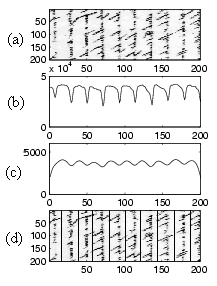
\includegraphics[width=0.5\textwidth]{fig1.png}
    \caption{(a) Một phần ảnh, (b) Hình chiếu, (c) Hình chiếu đã làm mịn, (d) Ảnh đã tách dòng}
    \label{fig:fig1}
\end{figure}

Kĩ thuật phân tách dòng mạnh mẽ với các biến thể kích thước dòng khác nhau và đã được test trên nhiều trang viết tay. Bước tiếp theo sau phân tách dòng là tạo scale space của ảnh cho blob analysis.

\subsection{Phân tích blob}
Bây giờ, chúng ta sẽ xem xét ảnh từng dòng độc lập để lấy ra từ. Ảnh một từ được tạo ra bởi các kí tự rời rạc, các kí tự có kết nối với nhau, hoặc kết hợp của cả 2. Chúng ta sẽ muốn kết hợp các sub-unit đó lại trong 1 đối tượng word. Điều này có thể đạt được bằng cách tạo ra 1 biểu diễn blob-like của ảnh. Một blob có thể xem như một vùng liên kết trong không gian. Cách truyền thống để tạo ra blob là sử dụng Laplacian of Gaussian (LOG)[6], LOG là phép toán phổ biến và thường xuyên sử dụng cho xác định blobvà nhiều task phân tích ảnh multi-scale khác [2, 6]. Chúng ta sẽ sử dụng một biểu thức vi phân tương tự như LOG để tạo một biểu diễn multi-scale cho xác định blob. Tuy nhiên biểu thức vi phân của chúng ta khác ở chỗ chúng ta sẽ kết hợp đạo hàm từng phần bậc 2 the o2 hướng tại các scale khác nhau.

\subsubsection*{Non Uniform Gaussian Filters}
Trong phần này, một số tính chất đặc trung cho chữ viết được sử dụng để tạo nên phương pháp lọc từ. Trong [6] Lindeberg quan sát được rằng cực đại trong scale space xảy ra tại scale mà nó tỉ lệ với kích thước trong không gian của blob. Nếu quan sát một từ, có thể thấy rằng phạm vi không gian của của từ được xác định:
\begin{enumerate}
    \item Từng kí tự xác định chiều cao của từ và
    \item Chiều dài của từ xác định bởi số lượng kí tự.
\end{enumerate}
Một từ thường có nhiều hơn 1 kí tự và tỉ lệ chiều dài, rộng lớn hơn 1 (aspect ratio). Vì chiều $x$  của từ lớn hơn chiều $y$ nên tần số lọc không gian cũng nên cao hơn ở chiều $y$ so với chiều $x$. Kiến thức cụ thể về miền này cho phép chúng ta chuyển từ đẳng hướng(cùng scale trên 2 hướng) sang dị hướng. Chúng ta chọn chiều $x$  scale lớn hơn chiều $y$ để tương ứng với cấu trúc của từ. Gaussian filter dị hướng:

\begin{equation}
    G(x, y; \sigma_x, \sigma_y) = \frac 1{2\pi \sigma_x\sigma_y} e^{-(\frac {x^2}{2\sigma_x^2}+ \frac {y^2}{2\sigma_y^2})}~ (5)
\end{equation}

Chúng ta cũng có thể định nghĩa hệ số nhân $\eta = \frac {\sigma_x}{\sigma_y}$.

Trong phần lựa chọn scale, chúng tôi sẽ chỉ ra rằng aspect ratio trung bình hoặc $\eta$  nằm giữa 3 và 5 cho hầu hết tài liệu viết tay chúng tôi có. Thêm nữa, phản hồi của bộ lọc Gaussian dị hướng cũng đạt max trong khoảng này. Vi phân bậc 2 của Gaussian dị hướng được định nghĩa:

\begin{equation}
    L(x, y; \sigma_x,\sigma_y) = G_{xx}(x, y; \sigma_x, \sigma_y) + G_{yy}(x, y; \sigma_x, \sigma_y) ~(6)
\end{equation}

Một biểu diễn scale space của ảnh các dòng được tạo ra bằng cách tích chập ảnh với $(6)$. Ảnh đầu ra sẽ là:

\begin{equation}
    I(x, y; \sigma_x, \sigma_y) = L(x, y; \sigma_x, \sigma_y) \star f(x, y)~(7)
\end{equation}

Các đặc điểm chính lấy từ 1 biểu diễn scale space là blob-like(ví dụ: các vùng liên kết sáng hơn hoặc tối hơn so với background). Dấu của $I$ có thể được dùng để tạo ra 1 phân loại bề mặt cường độ thành tiền cảnh (foreground) và hậu cảnh (background). Ví dụ ảnh dòng trên hình~hình~\ref{fig:fig2}(a), hình~\ref{fig:fig2}(b), hình~\ref{fig:fig2}(c), hình~\ref{fig:fig2}(d), hình~\ref{fig:fig2}(e) là ảnh blob với scale tăng dần , ở \ref{fig:fig2}(b) với scale nhỏ thì hình chứa các blob kí tự, tăng scale lên thì là các blob từ. Điều này cho thấy hiện tượng các blob ghép lại với nhau. Tại một giá trị scale cụ thể thì blob khoanh vùng đúng vào các từ (hình~\ref{fig:fig2}(d)). Các scale lớn hơn là không cần thiết, nó sẽ khiến các blob các từ dính vào nhau hoặc làm tách blob của từ. Những hình ảnh này chỉ ra rằng có tồn tại một scale mà có khả năng khoanh vùng được hầu hết các từ. Trong phần tiếp theo, chúng tôi sẽ trình bày một cách tiếp cận để tự động chọn ra được scale thích hợp.

%ảnh 2
\begin{table}[ht]
\centering
\begin{tabular}{cc}
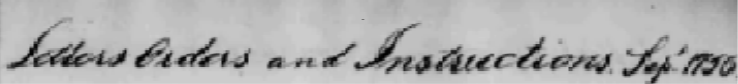
\includegraphics[scale=0.35]{imgs/a_line_img.png} & 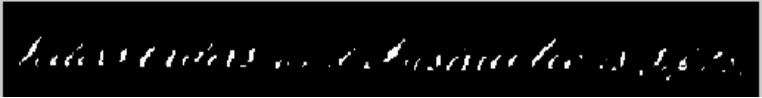
\includegraphics[scale=0.35]{imgs/bloby1x2.png} \\
(a) Ảnh gốc viết tay & (b) Ảnh blob với scale $\sigma_y = 1, \sigma_x = 2$ \\\\

\includegraphics[scale=0.35]{imgs/bloby2x4.png} & 
\includegraphics[scale=0.35]{imgs/bloby4x16.png} \\
(c) Ảnh blob với scale $\sigma_y = 2, \sigma_x = 4$ & (d) Ảnh blob với scale $\sigma_y = 4, \sigma_x = 16$\\\\

\includegraphics[scale=0.35]{imgs/bloby6x36.png}\\
(e) Ảnh blob với scale $\sigma_y = 6, \sigma_x = 36$
\end{tabular}
\captionof{figure}{Ảnh dòng chữ viết tay và đầu ra với các tỷ lệ khác nhau}
\label{fig:fig2}
\end{table}
%end ảnh 2

% HVN STARTS HERE
\subsection{Lựa chọn tỉ lệ}
Việc phân tích tỷ lệ khoảng cách không giải quyết được vấn đề lựa chọn tỷ lệ. Giải pháp cho vấn đề này phụ thuộc vào ứng dụng cụ thể và đồng thời phụ thuộc vào việc sử dụng thông tin trước đó để thực hiện quá trình lựa chọn tỷ lệ. Một phần trong công trình đề cập trong này được lấy cảm hứng từ quan sát của Lindeberg, ông cho rằng phản ứng từ cả tỷ lệ lẫn khoảng cách đạt mức lớn nhất khi giá trị của tỷ lệ sẽ tỷ lệ thuận với chiều của sự vật. Một tài liệu dạng ảnh bao gồm những cấu trúc như ký tự, các từ và dòng biểu diễn ở các tỷ lệ khác nhau. Tuy nhiên, khi so sánh với những loại ảnh khác, tài liệu dạng ảnh có những đặc tính riêng làm cho việc trích xuất một cấu trúc cụ thể không yêu cầu phải dùng nhiều giá trị tỷ lệ. Ví dụ, tất cả các từ chủ yếu có tỷ lệ tương đương nhau nên không cần phải chọn nhiều giá trị tỷ lệ. Từ đó, ta thấy rằng tồn tại một tỷ lệ mà từng từ riêng biệt sẽ hình thành một blob riêng. Sau đó đầu ra sẽ được tối ưu hóa ở giá trị tỷ lệ này. Các phân tích tiếp theo sẽ cho thấy rằng tỷ lệ này là một hàm theo chiều dọc nếu tỷ lệ khung hình là cố định.\par

Bây giờ chúng ta sẽ làm rõ sự khác biệt quan trọng giữa cách tiếp cận của Lindeberg và cách tiếp cận trong bài báo này. Ở công trình của Lindeberg, ông xác định độ lớn của tỷ lệ từ điểm cực đại thay vì ước lượng theo từng blob. Ông định nghĩa ước lượng blob bao gồm phạm vi không gian, độ tương phản và thời gian tồn tại. Một cấu trúc cây không gian tỷ lệ blob từ đó được hình thành để truy ra các blob đơn lẻ ứng với từng tỷ lệ. Phân tích chỉ ra rằng truy ngược từng blob riêng rẻ theo tỷ lẻ không phải là vấn đề liên quan cũng như khó có thể tính toán vì số lượng lớn các blob biểu diễn các ký tự và các từ. Đồng thời việc xác định liệu điểm cực trị ứng với một từ hay một ký tự cũng là điều không thể và như đã nêu trên thì tỷ lệ lý tưởng nhất cho một từ là một giá trị không hề lớn. Điều quan trọng ở đây là ta muốn ghép các blob ký tự lại với nhau để giới hạn lại blob từ. Từ đó, ta coi một blob là một vùng liên thông trên miền không gian và đo phạm vi không gian của blob đó. Phạm vi không gian là giá trị có thể tính toán được và ta quan sát thấy tham số này thay đổi theo tỷ lệ cực đại khi các blob ký tự được ghép với các blob từ. Điều này phù hợp với lý luận trực quan cho rằng khi tỷ lệ ở mức lý tưởng lúc quan sát thì mọi blob đều có một khoảng tỷ lệ (thời gian tồn tại) để tự biểu diễn.\par

Thuật toán trong bài báo này cần chọn ra $\sigma_y$ và hệ số nhân $\eta $ để trích xuất blob. Giá trị cực đại của phạm vi không gian của các blob chính là trường hợp lý tưởng nhất để tiến hành lọc, đây là phân tích giúp ta đưa ra được phương pháp chọn tỷ lệ đơn giản nhất. Để đo được độ thay đổi giữa phạm vi không gian của các blob so với tỷ lệ ta định nghĩa $\zeta_i$ đại diện cho khoảng rộng của blob thứ i. Như vậy tổng khoảng rộng của bộ blob A (tức một dòng) sẽ là $A = \sum_{i = 1}^{n} \zeta_i$.\par

\textbf{Lựa chọn $\eta$}. Tham số $\sigma_y$ và $\sigma_x$ sẽ có nhiệm vụ tìm được kích thước không gian của một từ. Một đặc tính quan trọng của một từ là tỷ lệ khung hình. Phân tích thủ công trên và bức ảnh cho thấy tỷ lệ khung hình trung bình của một văn bản dạng ảnh nằm trong khoảng $3.0 - 5.0$. Trước đó chúng ta đã định nghĩa hệ số nhân $\eta$ là $\sigma_x / \sigma_y$. Một phân tích khác trên vài bức ảnh khi để $\sigma_y$ là một hằng số ($\sigma_y$ không đổi) cho thấy cực trị của khoảng rộng khi áp dụng $\eta$ này nằm trong khoảng $3 - 5$. Ảnh một dòng chữ và phác đồ phân tích của ảnh được biểu diễn ở hình~\ref{fig:fig3}. Trong hình này, cực trị đạt được trong vùng 3.5 đến 4. Phân tích này cùng với quan sát cho thấy tỷ lệ khung hình trung bình của một từ nằm trong khoảng $3.0 - 5.0$ cho phép chúng ta chọn $\eta$ nằm trong khoảng này. Để phục vụ cho các phân tích tiếp theo thì ta chọn cụ thể là $\eta = 4$.

%ảnh 3
\begin{table}[ht]
\centering
\begin{tabular}{cM}
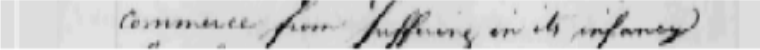
\includegraphics[scale=0.35]{imgs/a_line_img_1.png} & 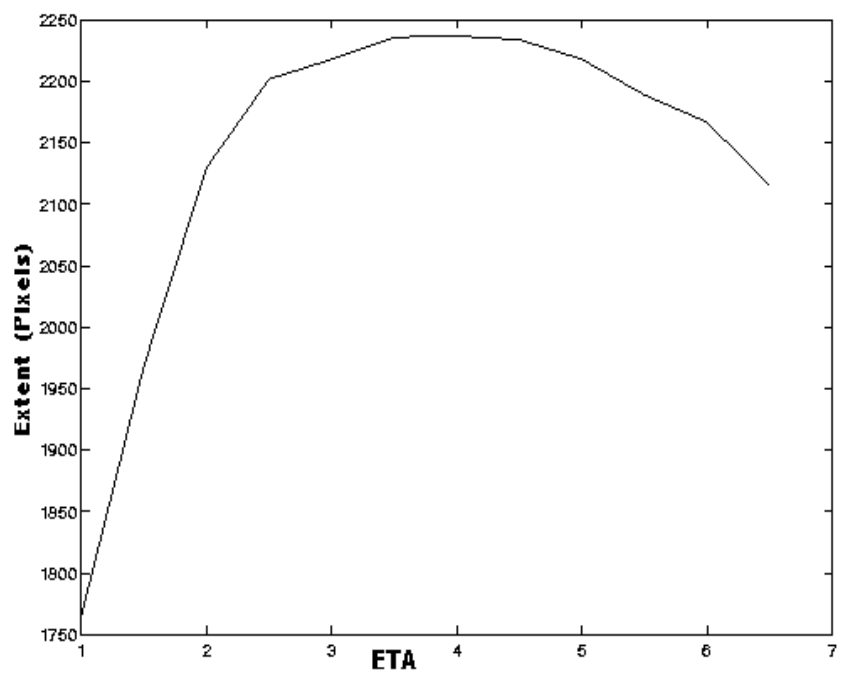
\includegraphics[scale=0.35]{imgs/ploty2n38.png} \\
(a) Ảnh gốc viết tay & (b) Đồ thị tương quan giữa khoảng rộng và $\eta$, trên ảnh này thì $\sigma_y = 2$, đạt cực trị khi $\sigma_y = 3.8$ \\
\end{tabular}
\captionof{figure}{Độ biến thiên của khoảng rộng blob và $\eta$ với $\sigma_y$ không đổi}
\label{fig:fig3}
\end{table}
%end ảnh 3

\textbf{Lựa chọn $\sigma_y$}. Như trong hình~\ref{fig:fig4}, tổng khoảng rộng có cực trị thay đổi khi $\sigma_y$ thay đổi nhưng $\eta$ không đổi. Hình~\ref{fig:fig4} cũng cho ta thấy cực trị đã bị dịch chuyển ra sao khi kích thước (cụ thể là chiều cao) của các ký tự thay đổi. Khi đưa vào thực nghiệm, ta phát hiện ra $\sigma_y$ là một hàm của chiều cao của các từ (điều này cũng cho thấy sự liên quan với chiều quan của cả dòng chữ). Ước lượng giá trị của $\sigma_y$ có thể suy ra được bằng cách dùng chiều cao của dòng chữ như sau.

\begin{equation}
\sigma_y = k \times \text{Chiều cao của dòng chữ}
\end{equation}

với $0 < k < 1$. Các giá trị tỷ lệ lân cận sau đó sẽ được kiểm chứng để xác định giá trị cực đại. Trong giai đoạn triển khai tác giả đã sử dụng $k = 0.1$ và thử nghiệm với $\sigma_y = 0.3$. Hai giá trị này đã được xác định khi thực nghiệm và cho ra kết quả khá tốt trên nhiều tập dữ liệu ảnh khác nhau.

%ảnh 4
\begin{table}
\centering
\begin{tabular}{MM}

\includegraphics[scale=0.35]{imgs/a_line_img_smaller_height.png} & 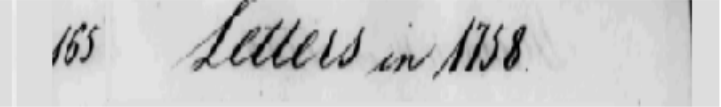
\includegraphics[scale=0.35]{imgs/a_line_img_larger_height.png} \\
(a) Ảnh gốc viết tay với chiều cao thấp & (b) Ảnh gốc viết tay với chiều cao cao hơn \\
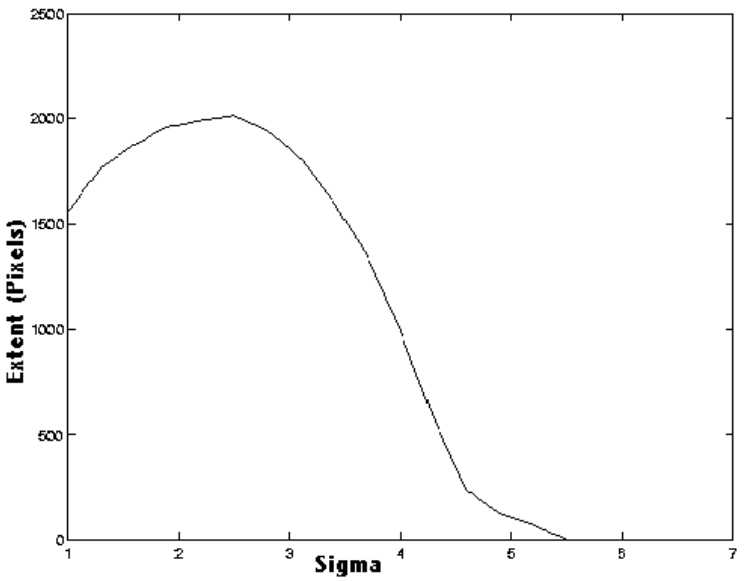
\includegraphics[scale=0.35]{imgs/ploty25n4.png} & 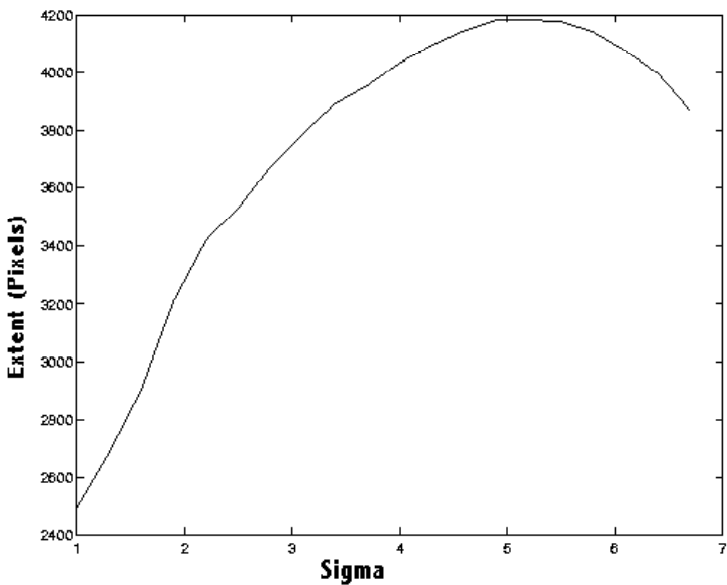
\includegraphics[scale=0.35]{imgs/ploty6n4.png}\\
(c) Đồ thị tương quan giữa khoảng rộng và $\sigma_y$, cực trị đạt được khi $\sigma_y = 2.5$ & (d) Đồ thị tương quan giữa khoảng rộng và $\sigma_y$, cực trị đạt được khi $\sigma_y = 6.0$
\end{tabular}
\captionof{figure}{Độ biến thiên của khoảng rộng blob và $\sigma_y$ với $\eta = 4$ không đổi.}
\label{fig:fig4}
\end{table}
%end ảnh 4

\subsection{Trích xuất blob và hậu xử lý}
Các blob sau đó sẽ được ánh xạ lại với ảnh gốc để xác định vị trí các từ. Một cách làm phổ biến chính là ghim blob vào một khu vực giới hạn (gọi là bounding box) được xác định thông qua phân tích các thành phần liên thông. Việc định vị khi biểu diễn từ bằng blob không được đảm bảo. Đồng thời một phần của các từ, đặc biệt là phần nhô lên và nhô xuống của chữ cái, sẽ bị lỗi do công đoạn tách dòng và làm mịn (làm mờ) ảnh trước đó. Vì lý do trên, bounding box sẽ được mở rộng để bao được hết phần nhô lên và nhô xuống đó. Đến giai đoạn này một bộ lọc bề mặt sẽ được sử dụng để loại bỏ đi các cấu trúc nhỏ do nhiễu ảnh.
% HVN ENDS HERE

\section{Kết quả}
Kỹ thuật này đã được thử nghiệm trên 30 bức ảnh được chọn ngẫu nhiên từ các phần khác nhau của các văn bản được viết bởi Geogre Washington (kho tài liệu với 6400 bức ảnh) và một số ảnh được lấy từ các văn bản do Eramus Hudson viết. Để giảm thời gian chạy, các bức ảnh đã được làm mịn và giảm kích thước xuống 1/4 so với kích thước ban đầu. Thuật toán mất 120 giây để có thể phân đoạn một trang tài liệu kích cỡ 800 x 600 pixels trên một máy tính với 200MHz pentium CPU và sử dụng hệ điều hành LINUX. Độ chính xác nằm trong khoảng 77\% đến 96\% và độ chính xác trung bình là 87.6\%. Hình~\ref{fig:fig5} cho thấy một phần của một bức ảnh đã được phân đoạn với hộp giới hạn được vẽ ứng với từng từ đã được phân tách. Phương pháp này hoạt động tốt trên cả nhưng bức ảnh bị mờ hay có nhiễu. Bảng~\ref{table:table4} thể hiện kết quả trung bình trên một bộ ảnh có 30 ảnh. Cột đầu tiên là số lượng từ trung bình trong một trang giấy được xác định bởi một người. Cột thứ 2 thể hiện tỉ lệ số từ được xác định bởi thuật toán (là các từ với hộp giới hạn bao quanh). Cột tiếp theo thể hiện tỉ lệ số từ bị phân mảnh. Một từ bị phân mảnh khi một chữ cái hay các chữ cái trong từ đó có hộp giới hạn tách biệt hay 50\% hoặc nhiều hơn số chữ cái trong từ đó không được phát hiện. Cột thứ 6 thể hiện các từ bị ghép vào với nhau, đây là các từ mà có chung hộp giới hạn. Cột cuối cùng thể hiện các từ đã được phân đoạn chính xác.

\begin{figure}
    \centering
    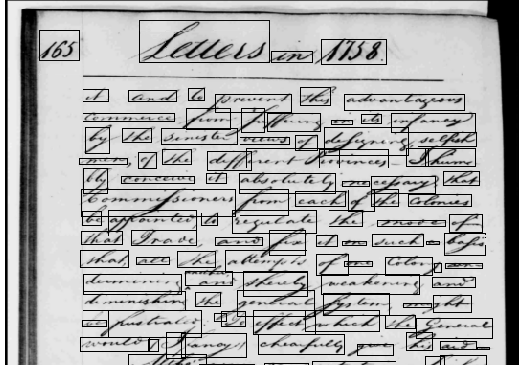
\includegraphics[width=0.8\textwidth]{fig5.png}
    \caption{Kết quả phân đoạn của một phần trong bức ảnh 1670165.tif được lấy từ bộ sưu tập Geogre Washington}
    \label{fig:fig5}
\end{figure}

\begin{table}
    \centering
    \begin{tabular}{|c|L|L|L|L|L|}
        \hline
        Số văn bản & Số từ trung bình trong 1 văn bản & \% các từ được xác định & \% các từ bị phân mảnh + dòng & \% các từ bị gộp & \% các từ xác định đúng \\
        \hline
        30 & 220 & 99.12 & 1.75 + 0.86 & 8.9 & 87.6 \\ 
        \hline
    \end{tabular}
    \caption{Bảng kết quả phân đoạn}
    \label{table:table4}
\end{table}

\section{Kết luận}
Chúng tôi đã thể hiện một kỹ thuật rất mới trong việc phân đoạn từ trong các văn bản viết tay. Thuật toán này của chúng tôi mạnh và hiệu quả bởi những lý do sau:
\begin{enumerate}
    \item Chúng tôi sử dụng các bức ảnh xám, do đó việc sử dụng ảnh trắng đen là không cần thiết. Việc chuyển đổi thành ảnh trắng đen cần lựa chọn ngưỡng kỹ lưỡng và nhìn chung là dẫn đến việc ảnh bị mất đi thông tin. Tham số ngưỡng cần phải được lựa chọn với từng bộ dữ liệu cụ thể và không thể sử dụng cho tất cả các bộ dữ liệu và nó rất nhạy cảm với nhiễu, mờ và các hiện tượng khác.
    \item Vì các bức ảnh đã được làm mịn cẩn thận và các blob không quan trọng có thể dễ dàng bị loại bỏ. Vì vậy kỹ thuật này tương đối không chịu ảnh hưởng bởi các hiện tượng nhiễu.
    \item Một lợi thế lớn trong cách tiếp cận này đó là phương pháp này không bị ảnh hưởng bởi hiện tượng loá. Lí do là bởi thuật toán này dựa trên làm mờ và thông tin được trích xuất dưới dạng blob.
    \item Thuật toán này đưa ra tối thiểu các giả định về bản chất của chữ viết tay và có thể được mở rộng sang phân đoạn từ trong các văn bản mà các từ không được phân đoạn bằng các dấu cách. Ngoài ra, phương pháp này không yêu cầu đào tạo trước.
\end{enumerate}

\section*{Trích dẫn}
\addcontentsline{toc}{section}{Trích dẫn}
\begin{thebibliography}{9}
    \bibitem{1}
    A.J. Robinson A.W. Senior. An off-line cursive handwriting recognition system. \emph{IEEE transactions on PAMI}, 3:309-321, 1998.
    
    \bibitem{2}
    D. Blostein and N. Ahuja. A multi-scale region detector. \emph{CVGIP}, 45:22-41, January 1989.

    \bibitem{3}
    R. G. Casey and E. Lecolinet. A survey of methods and strategies in character segmentation. \emph{IEEE Transactions on PAMI}, 18:690-706, July 1996.
    
    \bibitem{4}
    L. M. J. Florack. \emph{The Syntactic Structure of Scalar Images}. Kluwer Academic Publishers, 1997.

    \bibitem{5}
    J. Ha, R. M. Haralick, and I. T. Phillips. Document page decomposition by the bounding-box projection technique. In \emph{ICDAR}, pages 1119-1122, 1995.
    
    \bibitem{6}
    T. Lindeberg. \emph{Scale-space theory in computer vision}. Kluwer Academic Publishers, 1994.

    \bibitem{7}
    U. Mahadevan and R. C. Nagabushnam. Gap metrics for word separation in handwritten lines. In \emph{ICDAR}, pages 124-127, 1995.
    
    \bibitem{8}
    R. Manmatha and W. B. Croft. Word spotting : Indexing handwritten manuscripts. In Mark Maybury, editor, \emph{Intelligent Multi-media Information Re-trieval}. AAAI/MIT press, April 1998.

    \bibitem{9}
    G. Seni and E. Cohen. External word segmentation of off-line handwritten text lines. \emph{Pattern Recognition}, 27:41-52, 1994.
    
    \bibitem{10}
    S. Srihari and G. Kim. Penman : A system for reading unconstrained handwritten page images. In \emph{Symposium on document image understanding technology} (SDIUT 97), pages 142-153, April 1997.

    \bibitem{11}
    N. Srimal. Indexing handwritten documents, \emph{M.S. Thesis, University of Mas-sachusetts Computer Science Tech Report. 1999}.
    
    \bibitem{12}
    \emph{J. A. Weickert, S. Ishikawa, and A. Imiya. On the history of gaussian scale-space axiomatics. In J. Sporring, M. Nielsen, L. M. J. Florack, and P. Johansen, editors}, Gaussian Scale-Space Theory, \emph{pages 45-59. Kluwer Academic Press, 1997}. 
    
\end{thebibliography}

\end{document}